\documentclass{beamer}
\beamertemplatenavigationsymbolsempty
\usecolortheme{beaver}
\setbeamertemplate{blocks}[rounded=true, shadow=true]
\setbeamertemplate{footline}[page number]
\usepackage[utf8]{inputenc}
\usepackage{amsmath,amssymb}
\usepackage{hyperref}
\usepackage{biblatex}
\addbibresource{sample.bib}
\usepackage{array}
\usepackage{changepage}
\usepackage{caption}
\usepackage[T2A]{fontenc}
\usepackage[russian]{babel}
% Title Page Information
\title{Выбор оптимальной структуры модели глубокого обучения с контролем эксплуатационных характеристик}
\author{Фирсов Сергей }
\institute{Московский физико-технический институт}
\date{2024}

\begin{document}

\begin{frame}
    \titlepage
\end{frame} % 10 сек

%%%%%%%%%%%%%%%%%%%%%%%%%%%%%%%%%%%%%%%%%%%%%%%%%%%%

\begin{frame}{Цель исследования: }

\begin{itemize}
    \small
    \item \textbf{Neural Architecture Search:} 
    Метод автоматизированного поиска оптимальной архитектуры нейросети. 
    \item \textbf{Цель:} 
    Получать архитектуры решающие поставленную ML задачу, при этом удовлетворяя вычислительным или ресурсным ограничениям.
    \item \textbf{Проблемы:} % Challenges Проблемы //// 
    \begin{itemize}
        \footnotesize
        \item {Обширное пространство для поиска}
        \item {Баланс точности и сложности}
        \item {Получение семейства решений}
    \end{itemize}
    \end{itemize}
 
    \begin{figure}
        \centering
        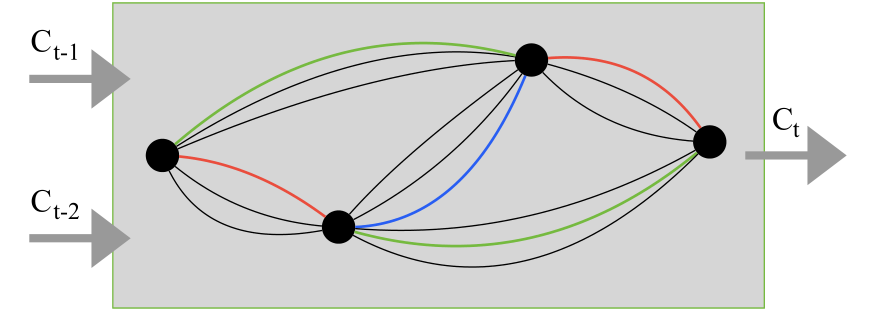
\includegraphics[width=0.5\linewidth]{Cells_DARTS_1_1.png}
        \caption*{Иллюстрация клетки из метода DARTS}
       
    \end{figure}
    

\end{frame} % 1 мин

% Здравствуйте, меня зовут Фирсов Сергей и я представляю Вам свою  работу на тему Выбор оптимальной структуры модели глубокого обучения с контролем эксплуатационных характеристик
% Объектом исследования является семейство методов NAS. Это  Методы автоматизированного поиска оптимальной архитектуры нейросети. 
% Наша задача ------- научиться получать архитектуры моделей \\ не только решающие поставленную задачу \\  но и удовлетворяющие поставленным вычислительным или ресурстным ограничениям
% Здесь можно выдвинуть несколько проблем \\
% Количество возможных архитектур растет !экспоненциально! по мере усложнения модели. \\
% Необходимо сбалансировать точность, сложностью и эффективностью модели на целевом оборудовании.
% Кроме того есть желаемое требование \\ получение в процессе обучения !семейства! решений зависящих от параметра сложности
% На рисунке иллюстрация взятого за основу метода DARTS, \\ в нём модель состоит из блоков, называемых клетками.\\ Каждая клетка содержит несколько вершин, отражающих состояния \\\\ и рёбер - отвечающих за возможные операции. \\ В процессе обучения происходит сэмплирование параметра сложности, по которому строятся архитектуры и обучаются веса,\\ дальше выбираются наиболее вероятные рёбра

% формализованная постановка задачи и предлагаемого метода представлена на слайде
% Хочу обратить внимание то что архитектурные параметры α мы предлагаем представить как функцию от параметра сложности S, \\ а этот параметр сложности \ вместо скалярного \ сделаем векторным, размерности количества операций \\ из соответствующего симплекса

% Итоговая задача оптимизации ставится как минимизация данного функционала: Мы сэмплируем вектора сложности,\ по которым строятся гиперсети генерирующие архитектуры. Они обучаются за счёт функции потерь задачи и регуляризационного члена 
% Кроме того добавим регуляризационный член, \\ позволяющий контролировать эксплуатационные характеристики
\begin{frame}{Постановка задачи} % == предлагаемый метод
\begin{itemize}
    \item Модель --- отображение $\mathbb{X} \times \Gamma \times \mathbb{W} \to \mathbb{Y}$, где $\gamma \in \Gamma$ задает вычислительный граф модели. 
    \item Будем задавать $\gamma \sim \textbf{GS}(\boldsymbol{\alpha}(\boldsymbol{S}, \boldsymbol{a}), t)$, а  архитектурные параметры \(\boldsymbol{\alpha}\) представим как функцию от \textbf{векторного} параметра сложности $ \boldsymbol{S}$ в пространство архитектур \(  \Gamma \):
    \[
    \boldsymbol{\alpha}: (\boldsymbol{S},\boldsymbol{a}) \to \Gamma, 
    \]
    где $ \boldsymbol{S} \in \Delta^{k-1}$ ---  \((k-1)\)-размерный симплекс,  \(k\) это количество операций, а \(\boldsymbol{a} \in \mathbb{R}^n\) --- параметры гиперсети. 
     
    
    \item \textbf{Оптимизационная задача:} минимизация функционала
    \begin{adjustwidth}{-1cm}{0cm} 
    $$\mathbb{E}_{\boldsymbol{S}\sim \boldsymbol{U}(\Delta^{k-1}) } \mathbb{E}_{\gamma\sim \textbf{GS} (\boldsymbol{\alpha}(\boldsymbol{S}, \boldsymbol{a}),t) }  \big[L(\boldsymbol{w}^*, \boldsymbol{\alpha}(\boldsymbol{S},\boldsymbol{a})) + \kappa \cdot \text{Lat}(\boldsymbol{\alpha}(\boldsymbol{S},\boldsymbol{a})))\big] \to \min\limits_{w,\boldsymbol{a}},
    $$\\
    где $\text{Lat}(\boldsymbol{\alpha}(\boldsymbol{S}, \boldsymbol{a})))$ --- регуляризационный член отвечающий за сложность модели и задержку выполнения операций
    \end{adjustwidth}
\end{itemize}


    
\end{frame}
%%%%%%%%%%%%%%%%%%%%%%%%%%%%%%%%%%%%%%%%%%%%%%%%%%%%

% Ещё пару слов об архитектуре решения: компоненты векторного параметра сложности можно воспринимать как коэффициенты регуляризации по соответствующим операциям. Таким образом задавая вектор с большим штрафом за пуллинг - мы ожидаем увидеть меньше таких операций в модели, 
\begin{frame}{Архитектура решения}
\includegraphics[width=1\linewidth]{Idea.png}
\centering
\small Рис. 2: Иллюстрация предлагаемого метода.
\begin{itemize}
    \item Предлагается использовать векторный параметр сложности $\boldsymbol{S}$, компоненты которого --- коэффициенты регуляризации по соответствующим операциям
    \item Гиперсеть на основе $\boldsymbol{S}$ генерирует архитектурные параметры для нейросети
\end{itemize}
\end{frame}


%%%%%%%%%%%%%%%%%%%%%%%%%%%%%%%%%%%%%%%%%%%%%%%%%%%%


\begin{frame}{Постановка эксперимента}
\begin{itemize}
    \item Цель эксперимента – проверка работоспособности предлагаемого метода, качества получаемых моделей и возможности контроля эксплуатационных характеристик.
    \item Эксперимент проводится на выборке Fashion-MNIST.
    \item Модель состоит из трех ячеек, в каждой по 4 вершины. 
    \item Во время обучения температура распределения гумбель-софтмакс понижалась от 1 до 0.2. % надо ли? ещё что-то написать? количество эпох

\end{itemize}
\end{frame}

%%%%%%%%%%%%%%%%%%%%%%%%%%%%%%%%%%%%%%%%%%%%%%%%%%%%


\begin{frame}[t]{Результаты}
% на данном слайде показаны результаты работы метода и примеры трёх полученных моделей
% В данной конфигурации \\ модели на выбор даётся всего 3 операции - ......... и соответственно рассмотрим 3 случая. Одинаковый штраф - вектор сложности  такой, увеличенный штраф за свёртки -.. или за пулинг
% Мы можем видеть работоспособность предлагаемого метода. Когда штрафуем за пулинг - исчезают операции соответствующего типа, когда за счёртку - аналогично. 
% Таким образом предлагаемый метод позволяет контролировать сложности модели - отражением которой считаем количество параметров или другие эксплуатационные характеристики - к примеру задержку выполнения операций. Зная что свёртка вычисляется в несколько раз дольше пулинга - можно изменив вектор сложности получить более быструю модель
\begin{minipage}[t][0.4\textheight]{\textwidth}  
  \begin{columns}[T, totalwidth=\textwidth]
    \begin{column}{0.3\textwidth}
    \centering
    1. Одинаковый штраф\\
    \textbf{0.33, 0.33, 0.33}\\ 
    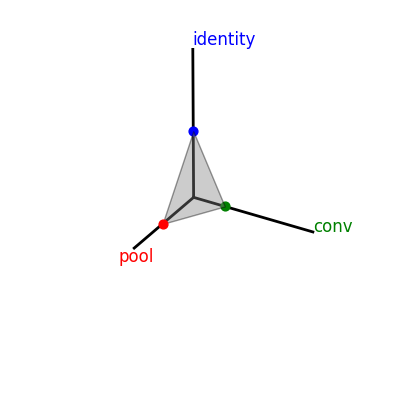
\includegraphics[width=\textwidth]{graf_1.png} 
    \end{column}

    \begin{column}{0.3\textwidth}
    \centering
    2. Увеличенный штраф за свёртки
    \textbf{0.15,0.15,0.70}\\
    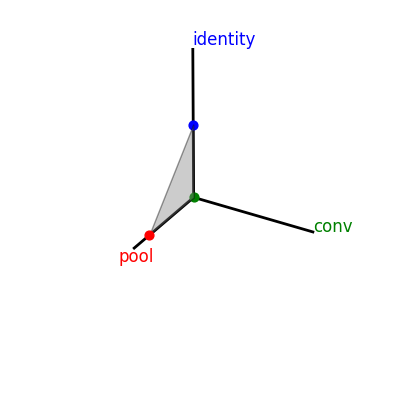
\includegraphics[width=\textwidth]{graf_2.png}
    \end{column}

    \begin{column}{0.3\textwidth}
    \centering
    3. Увеличенный штраф за пулинг
    \textbf{0.70,0.15,0.15}\\
    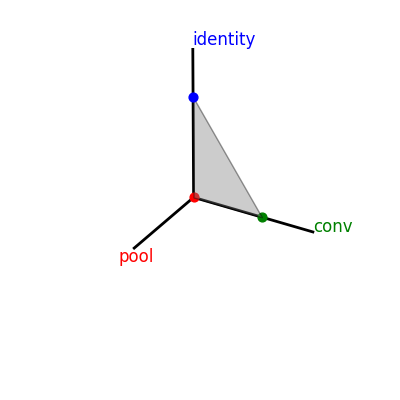
\includegraphics[width=\textwidth]{graf_3.png}
    \end{column}
  \end{columns}
\end{minipage}

\begin{minipage}[t][0.35\textheight]{\textwidth} 

  \begin{center}
     Рис 3. Иллюстрации распределения операций в моделях
  \end{center}


  \begin{table}[h!]
    \centering
    \small
   % \begin{tabular}{|c|c|c|c|}
    \begin{tabular}{b{4.5cm}|b{1cm}|m{1cm}|m{1cm}||}
    \hline
     \textbf{Модели} & 1 & 2 & 3 \\
    \hline
    \hline
    \textbf{Accuracy} &  82.5\% & 79.2\% &  85.0\% \\
    \hline
    \textbf{Количество параметров} & 38304 & 5120 & 143488 \\
    \hline
    \textbf{Количество pooling} & 12 & 17 & \textbf{0} \\
    \hline
    \textbf{Количество convolution} & 6 & \textbf{0} & 13 \\
    \hline
    \textbf{Количество identity} & 10 & 11 & 15 \\
    \hline
    \end{tabular}
  \end{table}
\end{minipage}

\end{frame}




\begin{frame}{Результаты}
\begin{itemize}
    \item Предложен метод позволяющий получать семейство моделей с возможностью контроля сложности обучения и аппаратных ограничения.
    \item Метод обладает возможностью получать архитектуры моделей за счёт изменения вектора параметра сложности без необходимости дополнительного дообучения.
    \item Вычислительные эксперименты подтверждают работоспособность метода и демонстрируют заявленную гибкость получаемого решения.
\end{itemize}
\end{frame}


\begin{frame}[allowframebreaks]{References}
    \tiny
    \nocite{*}
    \printbibliography
\end{frame}
% ------------------------------------------------------------


\end{document}

